\section{Electrodiffusion in the extracellular space}
\label{sec:Eldiff}
\index{Electrodiffusion}


In this Chapter we will explore the effects that diffusion may have on extracellular potentials. To do this, we will use the two-step, Hodgkin-Huxley-Cable + Kirchhoff-Nernst-Planck (HHC+KNP) scheme. This scheme was briefly introduced in Section \ref{sec:Schemes:KNP}, but we shall present it in further detail in this chapter. As we explained earlier, the HHC+KNP scheme allows us to combine simulations of morphologically detailed neurons (Step 1) with electroneutral electrodiffusive dynamics of the ion concentrations $c_k$ and electric potential $\phi$ in the extracellular space (Step 2). 

In Step 1, the (HHC-type) neurodynamics is computed under the assumption that it is independent of whatever goes on in the extracellular space. We shall in the following assume that the neurodynamics is known, and expressed as a set of transmembrane ion specific sources ($f_k$) and an additional capacitive neuronal membrane current source density ($f_{cap}$). These variables, along with other relevant variables, will be defined properly below (Section \ref{sec:Eldiff:porous}). 

In Step 2, the neuronal transmembrane output is treated as distributed "external input" to the extracellular medium. The KNP scheme is then used to compute the resulting dynamics of $c_k$ and $\phi$. As we explain below (Section \ref{sec:Eldiff:porous}), we shall describe the extracellular dynamics on a coarse-grained scale, and treat the extracellular medium as a continuous, porous medium.

\subsection{\blue{Continuous, porous medium approximation for electrodiffusion}}
\label{sec:Eldiff:porous}
\index{Continuous medium}
\index{Porous medium}
In Chapter \ref{sec:Sigma}, we introduced the continuous, porous medium approximation for coarse grained volume conduction in brain tissue. A similar approximation can be used for extracellular electrodiffusive processes following the KNP scheme. 


Unlike what we did in Chapter \ref{sec:Sigma}, where our reference volume was the tissue as a whole, we shall here follow the convention that we use only the fraction $\alpha$ of tissue that is extracellular space as our reference volume \citep{Sykova2008}. 

If we define all extracellular variables relative to the extracellular volume fraction  (Fig. \ref{Eldiff:fig:porous}), they can be defined as:

\begin{figure}[!ht]
\begin{center}
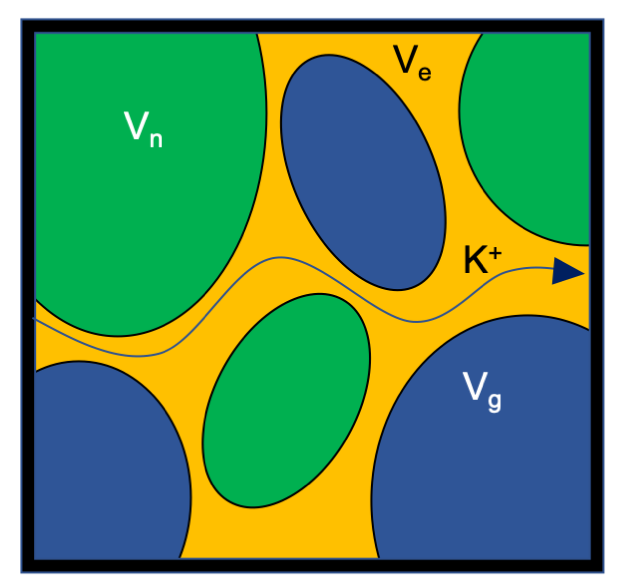
\includegraphics[width=0.5\textwidth]{Figures/Eldiff/Porous.png}
\end{center}
\caption{\textbf{Tortuous, porous medium.}  Sketch of a cross-section of a piece of neural tissue. Extracellular space (orange) occupies a fraction $\alpha$ (about 0.2 of the total tissue volume), while neurons and glial cells occupy about equally much of the remaining space. The extracellular space has a highly tortuous structure. We consider tissue transport processes that are confined to occur only in the extracellular part of the tissue. Detours around neuronal and glial obstacles are accounted for by the tortuosity $\lambda$. 
\tvnnote{kanskje med panel B en zoomet ut versjon der det ser mer homogent ut? Hadde Klas allerede laget en lignende figur til Sterratt? Dette bildet overdriver forresten situasjonen litt, siden det er fryse-tørket eller noe slikt, så mesteparten av CSFen er tatt bort.}
}
\label{Eldiff:fig:porous}
\end{figure}

\begin{itemize}
\item $c_k$ (units $\mathrm{mol/m^3}$ = mM) is the extracellular concentration of an ion species $k$, defined as the number of extracellular ions of species $k$ (in mol) per extracellular volume unit (which is a fraction $\alpha$ of the tissue volume unit).

\item $\rho_e$ (units $\mathrm{C/m^3}$) is the extracellular charge density
concentration of an ion species $k$, defined as the number of extracellular ions of species $k$ (in mol) per extracellular volume unit (which is a fraction $\alpha$ of the tissue volume unit).

\item ${\bf j_k}$ (units $mol/\mathrm{m^2s}$) is the extracellular flux density of an ion species $k$, defined as the number of extracellular ions (in mols) crossing an extracellular unit cross- section area (which is a fraction $\alpha$ of a unit tissue cross-section area) per second.

\item  ${\bf i_e}$ (units $\mathrm{A/m^2}$) is the extracellular current density, defined as extracellular current per per extracellular unit cross-section area. In comparison, the current density ${\bf i}$ in Chapter \ref{sec:VC} was defined as extracellular current per unit tissue cross-section area, which means that ${\bf i_e} = {\bf i}/\alpha$.

\item $\tilde{D}_k$ (units $\mathrm{m^2/s}$) is the effective diffusion constant \index{Diffusion constant} for ion species $k$ in the extracellular medium. It is defined so that the diffusive flux is given by ${\bf j_k^{diff}} = -\tilde{D}_k \nabla c_k$ \citep{nicholson2001}. The effective diffusion constant accounts for the fact that diffusing ions face obstacles (neurites) along their path forcing them take detours, reflected through a tortuosity $\lambda$ which has a value of about 
$1.6$ in the extracellular space \citep{Nicholson1998}. The effective diffusion constant is given by:
\begin{equation}
\tilde{D_k} = \frac{D_k}{\lambda^2}, 
\label{Eldiff:eq:diffconst}
\end{equation}
where $D_k$ is the diffusion constant for an ion species $k$ in the pure (unhindered) extracellular solution. The fact that diffusing ions are confined the stay only in the extracellular volume fraction $\alpha$ is already accounted for in the flux definition. 

\item $\sigma_e$ (units S/m) is the tissue averaged extracellular conductivity for extracellular current densities defined as ${\bf i_e}$. As we show later, $\sigma_e$ can be expressed as a function of ion concentrations:
\begin{equation}
\sigma_e = \frac{F}{\psi}\sum_{k} \tilde{D}_k z_{k}^2 c_{k}.
\label{Eldiff:eq:sigma1}
\end{equation}
Here $z_{k}$ is the valency of ion species $k$, and $\psi=RT/F$ is defined by the gas constant ($R$), Faraday's constant ($F$) and the temperature ($T$). Since $\sigma_e$ relates to ${\bf i_e}$ in the same way that $\sigma$ related to ${\bf i}$ in Chapter \ref{sec:VC}, $\sigma_e = \sigma /\alpha$.

\item $f_k$ (units mol/m$^3$) is the ion-flux-source density, i.e., the local neuronal output of an ion species $k$ per per extracellular volume unit. It is essentially is the ion-dynamics counterpart to the current-source-density (CSD) presented earlier (eq. \ref{VC:eq:CSD1}).

\item $C_e$ (units A/m$^3$) is the current source density, i.e., the local neuronal output current per extracellular volume unit. $C_e = C/\alpha$ where $C$ (as defined in Chapter \ref{sec:VC}) is neuronal output current per tissue volume unit.
\end{itemize}


\subsection{\blue{Electrodiffusive ion concentration dynamics}}
\label{sec:Eldiff:ionconcentrationdynamics}
In the coarse-grained description, using the effective diffusion constant, $\tilde{D}_k$, the flux density (${\bf j_k}$) of an ion species $k$ is given by the Nernst-Planck equation:
\begin{equation}
{\bf j_k} = - \tilde{D}_k {\bf \nabla} c_{k} - \frac{\tilde{D}_k z_k c_k}{\psi} {\bf \nabla} \phi.
\label{Eldiff:eq:JNP}
\end{equation}
The first term on the right hand side of eq. \ref{Eldiff:eq:JNP} is the ionic flux density due to diffusion (${\bf j_{k}^\text{diff}}$), and the second term is the additional flux density due to electrical drift along gradients in the extracellular potential $\phi$ (${\bf j_{k}^\text{drift}}$). 

The general continuity equation for an ion species $k$ is,
\begin{equation}
\frac{\partial c_k}{\partial t} = - \nabla \cdot {\bf j_k} + f_k,
\label{Eldiff:eq:salamander}
\end{equation}
where we have included the neuronal source term $f_k$. If we insert the electroduffusive flux density (eq. \ref{Eldiff:eq:JNP}) into eq. \ref{Eldiff:eq:salamander},
we get the Nernst-Planck continuity equation:
\begin{equation}
\frac{\partial c_k}{\partial t} = {\bf \nabla} \cdot \left[ \tilde{D}_k {\bf \nabla} c_k + \frac{\tilde{D}_k z_k c_k}{\psi} {\bf \nabla} \phi \right] + f_k.
\label{Eldiff:eq:NP}
\end{equation}
This equation was listed earlier (eq. \ref{Schemes:eq:NPe}) as the fundamental equation in the KNP scheme. Eq. \ref{Schemes:eq:NP} gives us one equation for each individual ion concentration $c_k$, and to solve the system of equations, we are in need an additional equation for the additional variable $\phi$. 


\subsection{\blue{Electrodiffusive electrodynamics}}
\label{sec:Eldiff:electrodynamics}
From the equations for ion concentration dynamics (eqns. \ref{Eldiff:eq:JNP}-\ref{Eldiff:eq:NP} ) we can derive a corresponding set of equations for net charge dynamics. This will show us how they relate to to the VC theory presented in Chapter \ref{sec:VC}, and will also allow us to derive an expression for $\phi$.

If we multiply eq. \ref{Eldiff:eq:JNP} by $F\cdot z_k$ and sum over all ion species $k$, we get the extracellular current density:
\begin{equation}
{\bf i_e} = F\sum_k {z_k {\bf j_k}} = -\sum_k{F z_k \tilde{D_k}{\bf \nabla} c_{k}} - F\sum_{k} \frac{\tilde{D_k} z_{k}^2}{\psi}c_{k} {\bf \nabla}{\phi}, 
\label{Eldiff:eq:INPa}
\end{equation}
where the first term on the right hand side is the diffusive current density ${\bf i_e^\text{diff}}$, and the second term is the Ohmic drift current density ${\bf i_e^\text{drift}}$. Since we know from earlier that the drift current density should equal $- \sigma_e \nabla \phi$  (cf. eq. \ref{VC:eq:ohmici}) we may identify the the conductivity $\sigma_e$ of the extracellular medium as \citep{Koch1999}:
\begin{equation}
\sigma_e = \frac{F}{\psi}\sum_{k} \tilde{D}_k z_{k}^2 c_{k},
\label{Eldiff:eq:sigma}
\end{equation}
as we postulated in eq. \ref{Eldiff:eq:sigma1}. With this, we can write eq. \ref{Eldiff:eq:INPa} on the simpler form:
\begin{equation}
{\bf i_e} = - \sum_k{F z_k \tilde{D_k}{\bf \nabla} c_{k}} - \sigma_e{\bf \nabla}{\phi},
\label{Eldiff:eq:INP}
\end{equation}

Likewise, if we multiply eq. \ref{Eldiff:eq:salamander} by $F\cdot z_k$ and sum over all ion species, we get the continuity equation for charge: 
\begin{equation}
\frac{\partial \rho_e}{\partial t} =  \nabla \cdot \left (\sum_k{F z_k \tilde{D_k}{\bf \nabla} c_{k}} + \sigma_e\nabla\phi  \right)  + C_e^{ion}.
\label{Eldiff:eq:chargecontinuity}
\end{equation}
We have here introduced the extracellular charge density (define as extracellular charge per tissue unit volume), 
\begin{equation}
\rho_e = F \sum_k z_k c_k + \rho_{0e},  
\label{Eldiff:eq:roen}
\end{equation}
and the ionic current source, 
\begin{equation}
C_e^{ion} = F \sum_k z_k f_k. 
\label{Eldiff:eq:csden}
\end{equation}
The term $\rho_{0e}$ in eq. \ref{Eldiff:eq:roen} represents a static extracellular charge density representing charged macromolecules and any species' of ions that are not included in the set $c_k$, and which is assumed to be constant in time and space. The index "ion" in eq. \ref{Eldiff:eq:csden} signifies that this source term exclusively accounts for the sources $f_k$ mediated by ions that pass through the neuronal membrane and enters or leaves the extracellular space in eq. \ref{Eldiff:eq:NP}. Importantly, $C_e^{ion}$ is not identical to the total CSD, which contains an additional capacitive component that accounts for the accumulation of a charge density $\rho_e^{mem}$ (defined as membrane charge per extracellular unit volume) at the exterior side of the neuronal membrane:
\begin{equation}
C_e = C_e^{ion} + C_e^{cap} = F \sum_k z_k f_k - \frac{\partial \rho_{e}^{mem}}{\partial t}.
\label{Eldiff:eq:CSDdecomposed}
\end{equation}
$C_e^{cap}$ interprets as the neuronal capacitive membrane current per extracellular unit volume (see Fig. \ref{Eldiff:fig:Ccap}), and the negative sign in front of the last term in \ref{Eldiff:eq:CSDdecomposed} follows from the fact that an outwards capacitive current (i.e., a source) implies an accumulation negative charge on the exterior side of the membrane. 

\begin{figure}[!ht]
\begin{center}
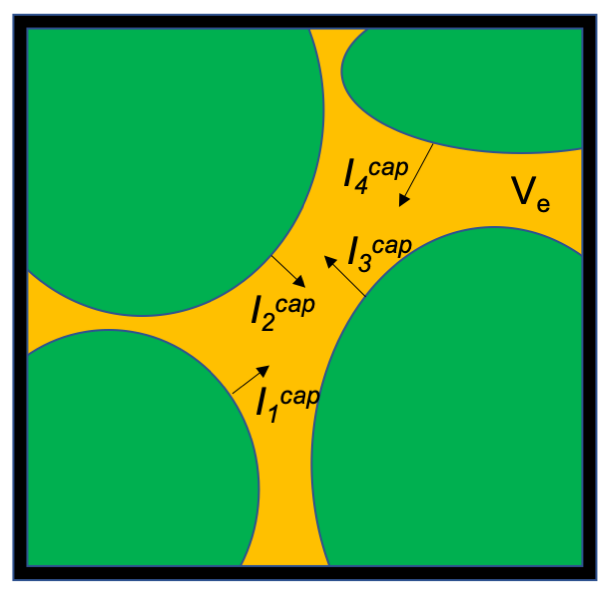
\includegraphics[width=0.5\textwidth]{Figures/Eldiff/KNP_Cap_illustration.png}
\end{center}
\caption{\textbf{Capacitive current sources}. Illustrated in terms of a finite volume of tissue, the capacitive current source density is the sum of capacitive currents entering the extracellular space from cells (green), divided by the fraction of the tissue volume that is extracellular (orange), i.e., $C_e^{cap} = \sum_k I_k^{cap}/V_e$. It can be interpreted as the accumulation of an extracellular charge density, which, since the bulk solution is assumed to be electroneutral, is associated exclusively by the charge accumulating at the exterior neural membranes.}
\label{Eldiff:fig:Ccap}
\end{figure}

Let us now look at the charge density, $\rho_e$ at the left hand side of eq. \ref{Eldiff:eq:chargecontinuity}. In general, $\rho_e$ could be composed of free charges in the extracellular bulk solution as well as charges bound to the outside of the neural membrane, i.e., we could have $\rho_e = \rho_e^{free} + \rho_e^{mem}$. However, as we have argued earlier, the bulk solution is very close to electroneutral, and if we assume perfect bulk electroneutrality ($\rho_e^{free} = 0$), we must have that $\rho_e=\rho_e^{mem}$. We can then combine eq. \ref{Eldiff:eq:chargecontinuity}  with eq. \ref{Eldiff:eq:CSDdecomposed} to arrive at:

\begin{equation}
\nabla \cdot (\sigma_e\nabla\phi) = - C_e - F \nabla \cdot \left (\sum_k{z_k \tilde{D_k}{\bf \nabla} c_{k}} \right).
\label{Eldiff:eq:eldiffCSD2}
\end{equation}

Eq. \ref{Eldiff:eq:eldiffCSD2} is the electrodiffusive counterpart to eq. \ref{VC:eq:CSD2}, that we used as starting point in standard VC theory. For a more direct comparison, we can multiply eq.  \ref{Eldiff:eq:eldiffCSD2} with the extracellular volume fraction $\alpha$, and get:
\begin{equation}
\nabla \cdot (\sigma\nabla\phi) = - C - F\alpha \nabla \cdot \left (\sum_k{z_k \tilde{D_k}{\bf \nabla} c_{k}} \right).
\label{Eldiff:eq:eldiffCSD22}
\end{equation}
Comparing eq. \ref{Eldiff:eq:eldiffCSD22} and eq.  \ref{Eldiff:eq:eldiffCSD2}, we see that the difference between them is the last term in eq. \ref{Eldiff:eq:eldiffCSD22}, which is the diffusive contribution not accounted for in \ref{VC:eq:CSD2}. As eq. \ref{Eldiff:eq:eldiffCSD2} shows, also diffusive processes can contribute to the genesis of extracellular potentials, and if present, they could give rise to a non-zero $\phi$ even in the absence of neuronal sources ($C = 0$). Diffusive currents can thus be seen as an additional "source" for generating extracellular potentials \citep{Halnes2017}. 

Provided that the neuronal current sources $C_e$ and the extracellular ion concentrations $c_k$ are known at a given time, eq. \ref{Eldiff:eq:eldiffCSD2} can be solved for $\phi$. In turn, the temporal development of $c_k$ are given by  the Nernst-Planck system of equations (eq. \ref{Eldiff:eq:NP}). Together, eqns. \ref{Eldiff:eq:NP} and \ref{Eldiff:eq:eldiffCSD2} are the fundament of the KNP scheme, which must be solved using some suitable numerical framework. 

In comparison, the standard VC-theory (assuming constant ion concentrations) is much easier to implement.  As we showed in Chapter \ref{sec:VC}), eq. \ref{VC:eq:CSD2} (which is eq.  \ref{Eldiff:eq:eldiffCSD22} without the last term) allows us to derive an analytical expression for the electrical potential at all points in space once the $C$ is known. 


\subsection{\blue{Do diffusion potentials matter?}}
\label{sec:Eldiff:estimates}
\index{Diffusion potential}
Due to the computational challenges they impose, it is tempting to make the assumption that diffusive currents contribute so little to the extracellular potential that we don't have to bother with them. This is what normally is being done, as most theoretical studies of extracellular potentials are based on standard VC theory. For most purposes, this is probably a good approximation, but its validity depends on one of the two following criteria being met:

\begin{enumerate}
\item C1: The magnitude of diffusive currents is much smaller than the magnitude of Ohmic drift currents.
\item C2: The frequency of diffusive currents is much lower than the frequency of the CSD and the Ohmic drift currents. 
\end{enumerate}

The first criterion is general and quite intuitive. If C1 holds, the last term in eq. \ref{Eldiff:eq:eldiffCSD2} becomes much smaller than the other two terms, and standard VC theory will give accurate predictions of $\phi$. As we shall see below, it is quite likely that C1 is violated under many physiological conditions. If so, the second criterion (C2) may still come to our rescue. In most experiments, extracellular potentials are recorded using electrode systems with a lower cut-off frequency of 0.1-1 Hz \citep{Einevoll2007}. As diffusive currents are proportional to concentration gradients, which generally vary at a much slower time scale than $\phi$, diffusive contributions to $\phi$ are often direct-current (DC) like, i.e., they vary very slowly with time, and if they vary slowly enough, they will not be picked up in recordings using standard electrode systems, but only in experiments using DC electrodes. The question regarding their contribution to standard measurements is then whether they vary slowly enough. 

In the two following subsections we shall explore when and to which degree the criteria C1-C2 are likely to be met under physiological conditions.

\subsubsection{\blue{Magnitude of diffusion potentials.}}
To make some crude estimation of the magnitude that we can expect diffusion potentials to have in neural tissue, we make the following simplifications of eq. \ref{Eldiff:eq:eldiffCSD2}): Firstly, diffusion potentials depend solely on extracellular concentration gradients, and not on the instantaneous activity of neurons. Let us therefore assume that $CSD = 0$, and consider the extracellular dynamics is governed by:
\begin{equation}
\nabla \cdot (\sigma_e\nabla\phi_d) = - \nabla \cdot \left (\sum_k{F z_k \tilde{D_k}{\bf \nabla} c_{k}} \right), 
\label{Eldiff:eq:eldiffCSD3}
\end{equation}
where we have denoted the potential $\phi_d$ since, in this case, it will exclusively be evoked by diffusion. Let us further consider a system with closed boundaries, so that no current can enter or leave the system. In that case, we may simply skip the first nabla, and take:
\begin{equation}
\sigma_e\nabla\phi_d = -\sum_k{F z_k \tilde{D_k}{\bf \nabla} c_{k}}, 
\label{Eldiff:eq:diffpot}
\end{equation}
Essentially, eq. \ref{Eldiff:eq:diffpot} states that the Ohmic drift current and diffusive current must cancel each others at each point in space, i.e., that if no current enters the system from the outside, no net current should be observed anywhere inside the system. The diffusion potential is thus the potential that we must have in the system for this to be the case. 

Finally, due to the linearity in eq. \ref{Eldiff:eq:diffpot}, the diffusion potential between two points in space is a direct function of the the ionic concentrations at these two points. Hence, it is sufficient for our task to consider a simple two-compartment system (like that in Fig. \ref{Schemes:fig:diffpot}). For two-compartment systems, eq. \ref{Eldiff:eq:diffpot} further simplifies to:

\begin{equation}
\Delta \phi_d = \frac{F}{\bar{\sigma_e}} \sum_k{z_k \tilde{D}_k \Delta c_k}
\label{Eldiff:eq:diffpot2}
\end{equation}
where $\Delta c_k = c_{k}^{2} - c_{k}^{1}$ and $\Delta \phi_d = \phi_d^{2} - \phi_d^{1}$ denote the concentration and potential difference between compartments 1 and 2. Within each compartment, $\sigma_e$ can be determined from the ionic concentrations by use of eq. \ref{Eldiff:eq:sigma1}. However, since we for this problem need the conductivity experienced by an Ohmic current traveling between the two compartments, we have in eq. \ref{Eldiff:eq:diffpot2} used the average $\sigma_e$ of the two compartments:
\begin{equation}
\sigma_e = \frac{F}{2\psi}\sum_{k} \left(\tilde{D}_k z_{k}^2 c_{k}^{1} + \tilde{D}_k z_{k}^2 c_{k}^{2} \right).
\label{Eldiff:eq:sigma2}
\end{equation}

Based on eq. \ref{Eldiff:eq:diffpot2}, we make some estimates of the magnitude of the diffusion potential for some test examples.

\begin{itemize}

\item {\bf Diffusion potential under spreading depression:} The most extreme extracellular concentration shifts in the brain occur under the pathological condition called spreading depression, where the extracellular K$^+$ concentration can change by several tens of millomolars. In an an example from hippocampus, the K$^+$ concentration was about 30 mM higher at the bottom hippocampal layer than at the top hippocampal layer (Fig. 1a in \citep{Herreras1993}). In that experiment, only K$^+$ concentrations were recorded. However, we may give a crude estimate of the diffusion potential between the top and bottom of hippocampus by making some simple assumptions of the other ion concentrations: (i) We assume that the top layer of hippocampus remained at baseline concentrations. In the experiment, this seemed to be close to the case for $c_K$ \citep{Herreras1993}. In the top layer, we may therefore assume some rather typical baseline concentrations with $c_{Na} = 150$ mM, $c_{K} = 3$ mM and $c_{Cl} = 153$ mM. (ii) In the bottom layer, we assume that the $c_K$ was 30 mM above baseline, and that the increase in $c_K$ was compensated by an identical decrease in $c_{Na}$, so that electroneutrality was preserved. A plausible mechanism behind this would be that all concentration shifts were due to neuronal AP firing, i.e., neurons exchanging Na$^+$ for K$^+$. With these assumptions, we have $c_{Na} = 120$ mM, $c_{K} = 33$ mM and $c_{Cl} = 153$ mM in the bottom layer. Plugging the top layer and bottom layer concentrations into eq. \ref{Eldiff:eq:diffpot2}, we obtain a diffusion potential $\Delta \phi_d \sim 1$ mV across the hippocampal depth.

\item {\bf Diffusion potential in cortex during neuronal hyperactivity:} In several experimental papers, extracellular concentration shifts of selected ions have been recorded during induced neuronal hyperactivity and seizure activity \citep{kriv1975, nicholson1978, Dietzel1982, somjen1986, Dietzel1989}. The main focus of these works are typically on $c_K$, which is the most critical extracellular concentration due to its low baseline value. In these experiments, $c_K$ can typically change from a baseline value around 3 mM up to a ceiling level between 8-12 mM before the dynamics becomes pathological and is driven into spreading depression. Dietzel et al. estimated the concentration shifts in both $c_{K}$, $c_{Na}$ and $c_{Cl}$, and cased on a series of recordings, they estimated that the maximal diffusion potential that could be expected under their experimental condition was 0.4 mV \citep{Dietzel1989}.

\item{\bf Diffusion potential during normal activity:} It is difficult to find experimental data that allows us to estimate diffusion potentials in the brain under "normal" conditions, and the question as to whether concentration gradients are present in a given brain region probably depends on the processing state it is in. However, recordings from anesthetized cat cortex have shown that even during the resting state, $c_K$ may exhibit small-amplitude (0.5 mM) fluctuations \citep{MCCREERY1983}. In experiments recording the response in cortex to moderate (not seizure inducing) stimuli applied in the thalamus, cortical $c_K$ increases were found to have a depth profile, and vary by about 2 mM between different cortical layers \citep{Cordingley1978}. Thus, it seems likely that there should be some concentration gradients present in neural systems, and that e.g., a concentration difference of about 1 mM between the top and bottom of cortex or hippocampus would not be unlikely under normal processing. If we repeat the calculation from spreading depression, but assume that $c_{K}$ and $c_{Na}$ in the bottom layer were increased/decreased by 1 mM instead of 30 mM, we get a diffusion potential of about $33 \mu$V. This is of the same magnitude as potentials typically recorded in LFP recordings. 

\end{itemize}

Based on the crude estimates above, it is likely that many experimental conditions can contain diffusion potentials of the same magnitude as the potentials recorded in extracellular recordings, such as the LFP. 


\subsubsection{\red{GH: Frequency of diffusion potentials}}
\ghnote{Krevende kapittel. Sammenligne noen powerspectra her. Regne ut et par selv, ala Gratiy. Ser for meg at vi kanskje kjoerer eksemplene fra forrige delkap, og da lar konsentrasjonene falle til utjevining vha. diffusjon, samt et tilleggseksempel der vi lar dem falle eksponensielt med ulike tidskonstanter og bestemmer hvor raskt det maa gaa for at det skal fanges opp f.eks. ved 0.1 Hz. Da trenger vi paalitelige powerspectra fra eksperimentelle maalinger som vi kan sammenligne med. } 

Previous computational studies have predicted that effects of diffusion on extracellular potentials are not necessarily small, but tend to be very slow, meaning that they will only affect the very low-frequency components of $\phi$ \citep{Halnes2016, Halnes2017}. This is due to the diffusive current being a direct function of ion concentrations $c_k$, which on a large spatial scale typically vary on a much slower time scale (seconds-minutes) than the fluctuations in $\phi$ that we commonly are interested in (milliseconds-seconds). Furthermore, electrodes used to record $\phi$ typically have a lower cutoff frequency of 0.1-1Hz \citep{Einevoll2013}, which means that most of the tentative diffusive contribution will be filtered out from experimental recordings. It may therefore be a good approximation to neglect the diffusive term, except in the case of pathologically dramatic concentration variations.
